\documentclass[conference]{IEEEtran}

\ifCLASSINFOpdf%

\else

\fi


\usepackage{graphicx}
\usepackage{textcomp}
\usepackage{mathtools}
\usepackage[backend=bibtex, style=ieee]{biblatex}
\usepackage{tabularx, caption}
\usepackage{hyperref}
\usepackage{tikz}

\def\layersep{2.5cm}
\tikzstyle{neuron}=[circle,fill=black!25,minimum size=17pt,inner sep=0pt]
\tikzstyle{input neuron}=[neuron, fill=green!50]
\tikzstyle{output neuron}=[neuron, fill=red!50]
\tikzstyle{hidden neuron}=[neuron, fill=blue!50]
\tikzstyle{annot}=[text width=4em, text centered]

\addbibresource{bibliography}

\begin{document}

\title{Data Mining --- Flavours of Physics}

\author{\IEEEauthorblockN{Selene Baez Santamaria (2572529) \\
		Andrea Jemmett (2573223) \\
		Dimitris Alivanistos (2578740)}

\IEEEauthorblockA{
Vrije Universiteit Amsterdam \\
Amsterdam, Netherlands}}

\maketitle


\begin{abstract}
%TODO
\end{abstract}


\IEEEpeerreviewmaketitle%


\section{Introduction}
\label{sec:intro}
% different techniques can be applied in one problem and the best on os not often obvious.
\texttt{Kaggle} \footnote{\url{https://www.kaggle.com/}} is a crowdsourcing platform where data mining and machine learning techniques are applied on open ended problems. It is the largest and most diverse data community in the world. In early 2016, the European Organization for Nuclear Research (CERN) launched a competition regarding the detection of an undiscovered phenomenon, called the charged lepton flavour violation \cite{hirsch2011charged}.

The Standard Model of particle physics considers symmetry to be a crucial property. However in many proposed extensions of that model this symmetry does not exist, implying that decays that do not conserve lepton flavour are possible. Observation of this decay would be a clear indication of the violation of lepton flavour and a sign of long-sought new physics.

\subsection{Objectives}
The domain of particle physics is complex and has been slowly developing for the past decades. Incorporating this knowledge into data mining techniques can be time consuming, specially if the data scientists has no prior experience in the field.

%TODO explain transfer learning is one of the chosen techniques taht can easily be applied without domain knowledge

Hence, the two main objectives of this paper are:

\begin{itemize}
	\item To implement a classification tool, without any particle physics domain knowledge, that has comparable performance to classifiers submitted to the competition.
	\item Experiment with ensemble models and transfer learning.
\end{itemize}

\subsection{Research question}
\label{sec:researchQuestions}
The research question to be explored is \textit{How does an uneducated ensemble model perform in the aforementioned Kaggle competition? How does it accuracy compare to other more domain knowledgeable classifiers?}

\subsection{Hypothesis}
\label{sec:hypothesis}
We believe that data mining is powerful enough to achieve comparable performance even without domain knowledge. Yet, we recognize that achieving such accuracy requires proper tuning and a careful design of structures.

Our hypothesis is that by investing enough time in experimenting and fine tuning our model, a competitive score can be achieved. We measure the competitiveness by Kaggle's ranking system, and expect to rank among the top five competitors.

\subsection{Contribution}
Although perfect score has already been achieved in this competition, the use of domain knowledge was crucial for it. Thus the main contribution of this paper is to prove that advance data mining techniques can alleviate our score to the one that the winners accomplished.

Furthermore, if our hypothesis proves to be correct, this work could be a stepping stone for applying data mining techniques in complex domains where knowledge is incomplete or uncertain. It could show the potential of data mining, by discovering patterns and insights, to boost scientific advances.

\subsection{Organization}
This project follows the Cross Industry Standard Process for Data Mining (CRISP-DT) Framework. As such, this paper's sections correspond to the six phases of the process model.

Section ~\ref{sec:intro} has introduced some Business Understanding related to High Energy Physics, specifically the need for proving the violation of charged lepton flavour. Furthermore, Section~\ref{sec:related_work} explores different existing data mining approaches of Kaggle top competitors. We continue to gain some Data Understanding by describing the dataset and the competition tools and regulations in Section~\ref{sec:dataset}. The Data Preparation and Modeling steps are outlined in Section~\ref{sec:system_design}, where the data is cleaned and the model implementation is described. To Evaluate the classifier, we set up several experiments as depicted in Sections~\ref{sec:experiment} and ~\ref{sec:results}. Finally, Section~\ref{sec:conclusion} summarizes our observations throughout the process.

\section{Related Work}
\label{sec:related_work}
In order to develop our solution for this competition we studied the approaches of other participants. We focus on the winner's solution, since it achieved a perfect score, and on the fifth ranked solution, since it is similar to our chosen model.

\subsection{The Winner}
The winners of this competition were \textit{Vlad Mironov} and \textit{Alexander Guschin} of team Go Polar Bears. Their submission achieved 100\% accuracy by combining targeted solutions to the three main competition parts: improvement of the Area Under the Curve (AUC) score, and the given agreement and correlation tests.

Mironov and Guschin's model has two main characteristics to be noted. First, using scholar physics equations they recreated properties such as \textit{speed}, \textit{flight distance}, and \textit{mass}. This feature engineering step turned out to be crucial for the accuracy achieved. In fact, Vicens Gaitan, another participant ranked 14th in the competition, stated that other models, like Deep Networks, could build a mass-like property like the feature Mironov and Guschin engineered. Yet, Gaitan believes that the mass of a $\tau$ particle is hard to locate, even for this powerful methods.
%TODO add citation to his blog http://blog.kaggle.com/2015/10/27/passing-the-tests-strategies-used-in-cerns-flavour-of-physics/

Secondly, in order to significantly reduce the Mass correlation error, Mironov and Guschin used forests with \textit{Extreme Gradient Boosting}, a method used widely by data scientists to achieve state-of-the-art results on many machine learning challenges \cite{chen2016xgboost}. Parallelly, they used multilevel k-fold with bagging.

It is worth mentioning that the participants experimented with other configurations such as increasing the number of layers and neurons, however no significant changes in Area Under Curve were observed.

\subsection{Transfer learning solution}
The fifth ranked solution was submitted by Alexander Rakhlin and was based on transfer learning. This method assumes training and test data differ in some ways, a property extremely important for this competition. Furthermore, transfer learning does not require any prior domain knowledge but rather trains a model on a dataset and then applies the learned patterns to a different related one. This is a fundamental difference from the winners' solution, since the model is not tailored to the Physics domain and their features are not manually engineered.

A second highlight of this solution is the concept of ensemble neural networks. By combining the output of a large enough number of networks, a robust classifier is built. Furthermore, different from other solutions that output a result and then hope to pass the competition's tests, this model incorporates the three metrics (AUC and the agreement and correlation metrics) into the networks loss function. This ensures all of them are satisfied as result of statistical inference and not by coincidence.

\section{The Dataset}
\label{sec:dataset}
Given data from the Large Hadron Collider (LHC), proving the violation of the charged lepton flavour translates into a boolean classification task that determines the presence for the variable \textit{signal}.  The data has been collected directly at the
LHC during experiments with high energy particles collisions. The dataset consists of a collection of collision events and their properties. The objective of the competition is to predict whether a $\tau \rightarrow 3\mu$ decay (the one that identifies a lepton flavour) was present in the collision.

The competition provides a training and a test set, files to apply the agreement and correlation tests, as well as a format for submissions. A Starter Kit \footnote{\url{https://github.com/yandexdataschool/flavours-of-physics-start}} for different programming languages was made available, and the evaluation of them could only be done through the Kaggle platform.

\subsection{Training Data}
A ready-to-use labeled dataset was provided to use for training the classifier. The label, marked as \texttt{signal} is boolean where 1 identifies signal events while 0 represents background events. Signal events come from simulations. Background events come from real data collected by the LHCb, while observing collisions of accelerated particles with a specific mass range, in which $\tau \rightarrow 3\mu$, according to the Standard Model of particle physics, cannot happen.

The training dataset is given is CSV format and contains 49 features plus the target label. For a detailed description of the features see Appendix~\ref{sec:features}

\subsection{Evaluation requirements}
For this specific Kaggle competition the submission procedure is quite peculiar. Apart from the test set, the dataset comes with an \textit{agreement} and a \textit{correlation} set. In order for a submission to be scored on the test set, it needs to pass the agreement and correlation checks as a precondition.

\subsubsection{Agreement Test}
\label{sec:agreement}
Besides the presence of the $\tau \rightarrow 3\mu$ decay, there may be other obscure features that differentiate real from simulated data. Thus, it is possible for a classifier to reach high performances by picking up features that are not well modeled by the simulation. For this reason, contestants need to pass the Agreement Test.

The agreement dataset regards real and simulated events for an already known, observed and understood decay: $Ds \rightarrow \varphi\pi$. The control channel $Ds
\rightarrow \varphi\pi$ has similar properties as the $\tau \rightarrow 3\mu$ and may be present in real and simulated data. In order to apply the agreement test, all the training data provided contains the control decay signal, regardless of its origin, while it is completely absent in the test set. The \textit{Kolmogorov-Smirnov} test is used to evaluate the classifier distribution on real and simulated samples. Hence, in order to pass the agreement test, The Kolmogorov-Smirnov metric has to be smaller than 0.09.

\subsubsection{Correlation Test}
\label{sec:correlation}
In Physics, mass is not considered to be a reliable quantity to build a model around. For example, correlation with mass can cause artificial signal-like peaks or lead to incorrect estimation of background signals. For this reason it is important to check that the classifier's output is uncorrelated to the $\tau$ mass.

As such, the \texttt{mass} column is not included in the test dataset. However, there is hidden mass information that is used to perform a \textit{Cramer-von Mises} test. In sliding window fashion along the whole mass range, the CVM test iteratively compares the predicted values for entire dataset with the ones within a certain mass region. Getting similar distributions for all mass sub-regions means that the classifier is not correlated with the mass. Therefore, a well-designed classifier must yield to a value below 0.002 to pass the correlation test.

\subsection{Test Set}
\label{sec:test-set}
The test set has the same features as the training set has except for
\texttt{mass}, \texttt{production}, \texttt{min\_ANNmuon} and \texttt{signal}.
The data contained in this dataset consists of:
\begin{enumerate}
	\item simulated signal events for $\tau \rightarrow 3\mu$;
	\item real background events for $\tau \rightarrow 3\mu$;
	\item simulated events for the $Ds \rightarrow \varphi\pi$;
	\item real background events for $Ds \rightarrow \varphi\pi$.
\end{enumerate}

Events related to the control channel are not used for scoring, but only for the
agreement check (Section~\ref{sec:agreement}). One should treat all samples as
coming from the same collision channel during classification.

\subsection{Data preprocessing}
Since the goal of this project is to prove that domain knowledge is not necessary for achieving high accuracy in the posed classification task, we do not perform complex feature engineering. However, some data mining techniques, especially neural networks, are known to benefit from preprocessed inputs. As such, we perform basic preprocessing by removing the mean and scaling to unit variance.

\section{System Design}
\label{sec:system_design}
We build our model based on the Ensemble learning set of classifiers and apply
different variations and heuristics to the basic concepts, such as bagging and
stacking. The model consists of a composition of ensemble classifiers
implemented via Feed-forward Neural Networks, assembled together. The system
could be break down into two main stages: a first one where an ensemble of
Neural Networks is trained and used to produce predictions for all four datasets
(train, test, agreement and correlation); a second one where those predictions
are stacked with the original data to form an augmented dataset with as many new
features as networks in the first stage's ensemble (that is each data-point is
enriched with predictions from the ensemble).

The software implementation has been done in Python using a number of different
libraries for scientific computing (SciPy \cite{jones2015scipy} and
NumPy\footnote{\url{http://www.numpy.org/}}), dataset management, manipulation
and preprocessing (pandas\footnote{\url{http://pandas.pydata.org/}},
scikit-learn \cite{pedregosa2011scikit}) and neural networks model building,
training and evaluation (keras \footnote{\url{http://keras.io/}}). Keras is a
full-featured deep learning framework that is able to work seamlessly using
Theano \cite{bergstra2010theano} or TensorFlow \cite{abadi2016tensorflow} as
backends, on CPU or GPU without changing the source code.

\begin{figure}[h]
		\centering
		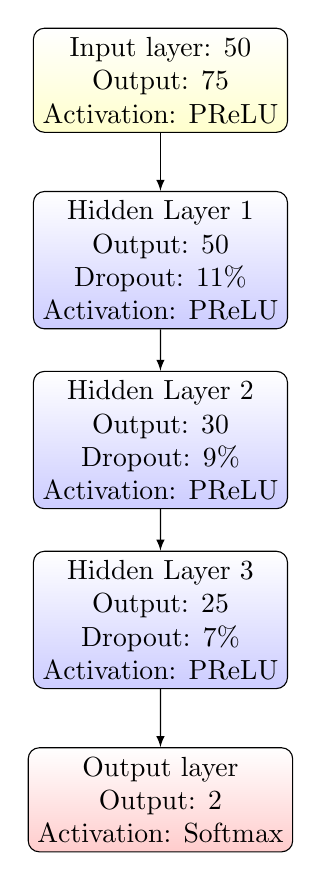
\begin{tikzpicture}[level distance=6.5em, edge from parent/.style={draw,-latex},
		every node/.style = {shape=rectangle, rounded corners, draw, align=center,
	top color=white, bottom color=blue!20}]]
			\node[bottom color=yellow!20] {Input layer: 50 \\ Output: 75 \\ Activation: PReLU}
			child { node {Hidden Layer 1 \\ Output: 50 \\ Dropout: 11\% \\ Activation: PReLU}
			child { node {Hidden Layer 2 \\ Output: 30 \\ Dropout: 9\% \\ Activation: PReLU}
			child { node {Hidden Layer 3 \\ Output: 25 \\ Dropout: 7\% \\ Activation: PReLU}
			child { node[bottom color=red!20] {Output layer \\ Output: 2 \\ Activation: Softmax}
			}}}};
		\end{tikzpicture}
		\caption{Neural Network configuration for the first stage (ensemble learning).}
		\label{fig:nn_ensemble_design}
\end{figure}

\subsection{Ensemble Neural Network Design}
\label{sec:NN_design}
Each neural network consists has the same specification, as given in Figure
\ref{fig:nn_ensemble_design}. It consists of 5 fully connected layers, the first
4 layers have a \textit{PReLU} activation function and the last one has a
\textit{softmax} one. The output layer has 2 outputs and this means that each
output represents the probability of the example being or not being a signal
respectively. We chose the \textit{PReLU} activation function because it is a
trainable parametric \textit{Rectified Linear Unit} (ReLU)  and so takes off the
burden of parameter tuning while leveraging an advanced and powerful activation
function, as demonstrated in \cite{he2015delving}. A rectified activation
function is of the form:
\begin{equation}
	f(y) = \begin{cases} y & \text{if } y > 0 \\ ay & \text{otherwise} \end{cases}
	\label{eq:relu}
\end{equation}
where $y$ is the input to the activation function and $a$ is a coefficient
controlling the slope of the negative part. When the coefficient is small, the
activation function is known as \textit{LeakyReLU} and while used to prevent
zero-gradients does not contribute to the performance of the model. The
coefficients in the PReLU, as explained in more detail in \cite{he2015delving},
can be learned jointly with the parameters of the model and the authors show
that it can outperform other rectified units with a number of different model.

Additionally, \textit{Dropout} is applied on the hidden layers in order to avoid
overfitting and prevent the complex co-adaptation in feature detectors (neurons) of a large neural network, as proved by \cite{srivastava2014dropout, hinton2012improving}. Particular attention is put in avoiding overfitting, because the performance of transfer learning at latter stages depends on it. Furthermore, Dropout helps to prevent the classifier from learning weakly simulated signals and pass the agreement and correlation
tests. Dropout is a simple technique consisting in randomly omitting or
disabling some neurons when a new training example is presented. The amount of
disabled neurons is directly controlled by an hyperparameter.

Training of the ensemble is done using only the training set and not the
agreement and correlation sets. We use the \textit{bootstrapping} technique,
which consists in using a different version of the dataset to train each network
in the ensemble that is obtained by sampling uniformly with replacement from the
original training set. It is commonly used to obtain an approximation of
independent and identically distributed predictions and is the first step
required to implement \textit{bagging}, a technique to reduce the variance of
the predictions distribution. Bootstrapping has been applied successfully to
ensemble of neural networks \cite{perrone1992networks, west2005neural}.

After experimentation, the chosen optimization algorithm is \textit{RMSProp}
\cite{tieleman2012lecture} and the loss function to minimize is given by the
\textit{categorical cross-entropy}. RMSProp is an adaptive learning rate
optimization method that performs generally well for deep networks, as
demonstrated in \cite{dauphin2015rmsprop, rudergradient, mnih2013playing}. Being
adaptive means that fine tuning of its hyperparameters (learning rate among
others) is a task with a lower priority than tuning, for example, dropout rates.
The cross-entropy is a statistical measure, borrowed from information theory,
formally defined over two distributions as the entropy of the first plus the
Kullback-Leibler Divergence between the first and the second, in formula:
\begin{equation}
	\mathcal{H}(p, q) = \mathcal{H}[p] + \mathcal{KL}(p||q)
	\label{eq:xentropy}
\end{equation}
It can be interpreted as the expected message-length per datum (in bits) when a
wrong distribution $q$ is assumed while the data actually follows a distribution
$p$. When used in data mining, the distribution $p$ represents the distribution
of labels in the training set, that is the true distribution, while the $q$
distribution represents the predicted labels. The cross-entropy then assumes the
following form:
\begin{equation}
	\mathcal{H}(y, \hat{y}) = -y \log \hat{y} - (1 - y) \log (1 - \hat{y})
	\label{eq:xentropy-dm}
\end{equation}
and is a quantity that we need to try to minimize.

After training is complete we generate predictions for all four datasets and
store them for the next stage. Predictions on the test set are also aggregated
using the mean to produce a \textit{majority vote} classification; this is a
simple implementation of bagging and unfortunately it is not sufficient to pass
the agreement and correlation tests.

\begin{figure}[h]
		\centering
		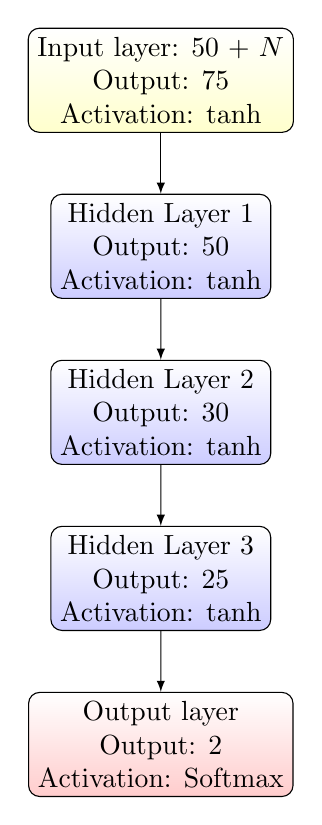
\begin{tikzpicture}[level distance=6em, edge from parent/.style={draw,-latex},
		every node/.style = {shape=rectangle, rounded corners, draw, align=center,
	top color=white, bottom color=blue!20}]]
			\node[bottom color=yellow!20] {Input layer: 50 + $N$ \\ Output: 75 \\ Activation: tanh}
			child { node {Hidden Layer 1 \\ Output: 50 \\ Activation: tanh}
			child { node {Hidden Layer 2 \\ Output: 30 \\ Activation: tanh}
			child { node {Hidden Layer 3 \\ Output: 25 \\ Activation: tanh}
			child { node[bottom color=red!20] {Output layer \\ Output: 2 \\ Activation: Softmax}
			}}}};
		\end{tikzpicture}
		\caption{Neural Network configuration for the second stage (transfer learning).}
		\label{fig:nn_trans_design}
\end{figure}

\subsection{Transfer Learning}
\label{sec:transductor}
In the second stage of training we create a single Neural Network with the
specifications given in Figure \ref{fig:nn_trans_design} and its weights are
initialized with a number of epochs of cross-entropy optimization on the
training data. Then an optimization algorithm (using SciPy and Powell's method)
is executed that tries to minimize a loss function that incorporates AUC on the
training set, Kolmogorov-Smirnov on agreement set and Cramer-von Mises on the
correlation set in the following way:
\begin{align}
	\mathcal{L} &= -\text{AUC} + \text{KS} + \text{CvM}
	\label{eq:loss}
\end{align}

The network is fed with the augmented data from the previous stage (original
data plus predictions from the previous stage) in order to implement stacking.
By doing this we aim at learning a better representation for the data. After
each optimization iteration we check whether the KS and CvM metrics are less or
equal to 0.09 and 0.002 respectively and that the AUC is greater than the
previous stored one. If all those three conditions are met, the network is
stored for later use (e.g. prediction).

Finally the generated ensemble of classifiers needs to be aggregated to form a
single prediction per data point. This is done again with the bagging technique,
by taking a majority vote (simple average in this case, because prediction
probabilities are required).

\section{Experimental set up and results}
\label{sec:experiment}
To evaluate and exploit the system proposed, different optimization algorithms, dropout rates and pre-trained epochs were tested. However, during all of these we kept some parameters statics.

First and foremost, during the ensemble stage we keep a constant number of $20$ neural network models trained for 75 epochs. The structure of each network is as explained in Section~\ref{sec:NN_design} and visualized in Figure ~\ref{fig:nn_ensemble_design}. During this stage a batch size of 64 is used for training and 256 for predicting. 

Secondly, during the transductor stage we have one neural network, as described in Section~\ref{sec:transductor} and visualized in Figure~\ref{fig:nn_trans_design}. We set the required thresholds for the agreement and correlation tests to $ks_threshold = 0.08$ and $cvm_threshold=0.002$. Moreover, we implement a stopping condition for producing only $30$ models, one at a time, which create predictions in order to try to pass the agreement and correlation test. 

\begin{figure}[!ht]
	\centering
	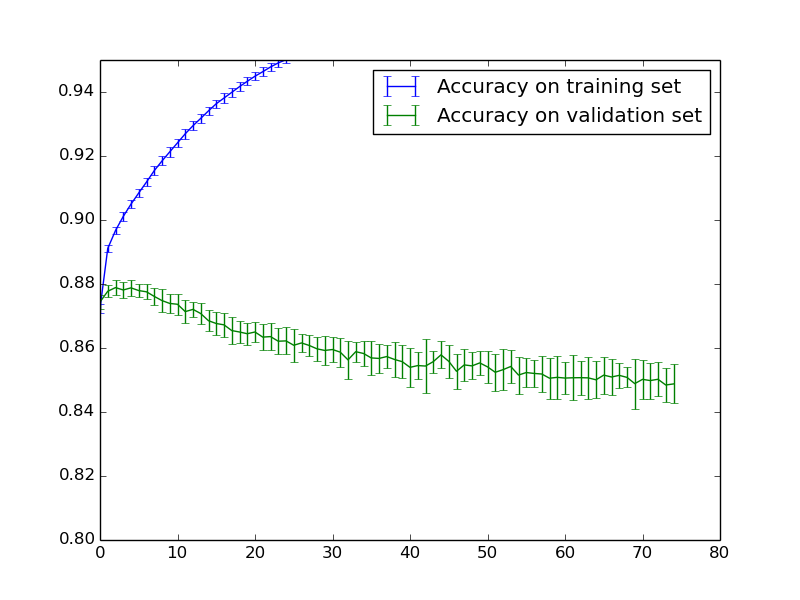
\includegraphics[width=.5\textwidth]{../imgs/ensemble_stats_d0.png}
	\caption{Performance of the ensemble of neural networks $0$ Dropout rate}
	\label{fig:dropout_0}
\end{figure}

\begin{figure}[!ht]
	\centering
	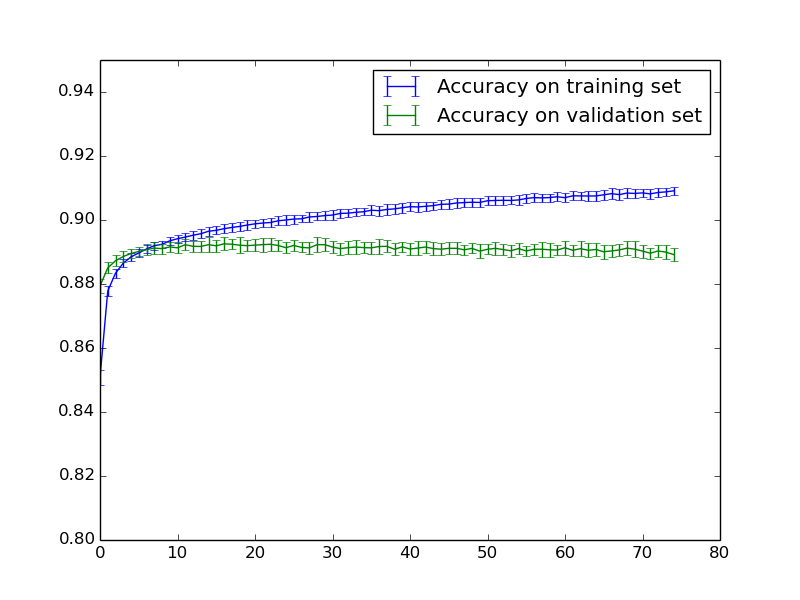
\includegraphics[width=.5\textwidth]{../imgs/ensemble_stats_d22.png}
	\caption{Performance of the ensemble of neural networks with homogeneous Dropout rate of $22$}
	\label{fig:dropout_22}
\end{figure}

\begin{figure}[!ht]
	\centering
	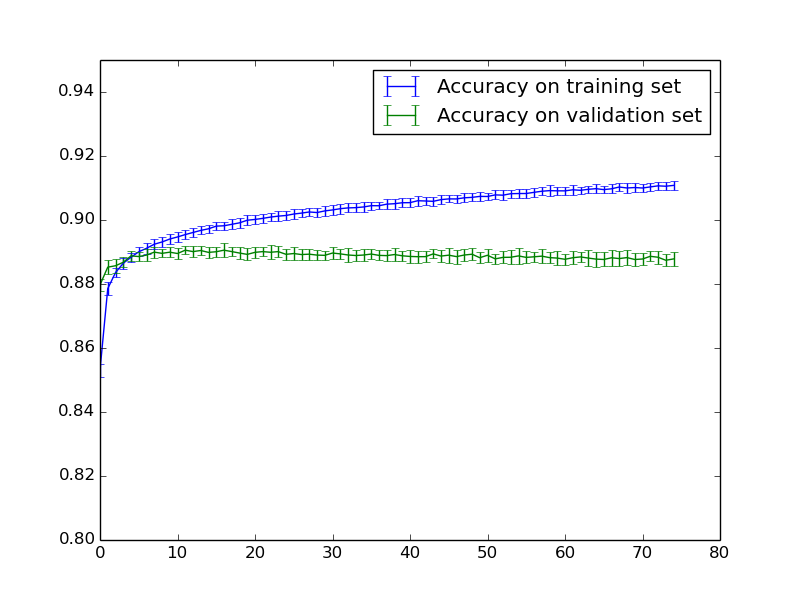
\includegraphics[width=.5\textwidth]{../imgs/ensemble_stats_d22_7.png}
	\caption{Performance of the ensemble of neural networks with heterogeneous Dropout rate of $22, 14.5 and 7$ }
	\label{fig:dropout_22_7}
\end{figure}

Given these static settings, we first experimented with different Dropout rates during the ensemble phase. Each rate was applied homogeneously to the first, second, and fourth hidden layers of each individual neural network. The third and fifth layers kept a static rate of $2$ and $4$ respectively. The rates tested were $0, 7, 11, and 22$. A special heterogeneous case was tested with rates $22, 14.5$ and $7$ applied to the dynamic layers.

Figures~\ref{fig:dropout_0} and ~\ref{fig:dropout_22} show the results from the two extreme values of Dropout rates in our experimentation, with the x-axis representing the number of epochs and the y-axis reflecting the accuracy achieved. On the one hand, not having Dropout leads to divergence in accuracy between training and testing sets. On the other hand, a rate as high as $22$ reduces the gap. This enhances the importance of avoiding overfitting. 

As for the difference between homogeneous and heterogeneous rates throughout the network, Figure~\ref{fig:dropout_22_7} shows that both settings have similar behaviors, with no significant improvement on introducing heterogeneity. As a result, we realize that fine tuning on Dropout rates is not necessary.

\begin{figure}[!ht]
	\centering
	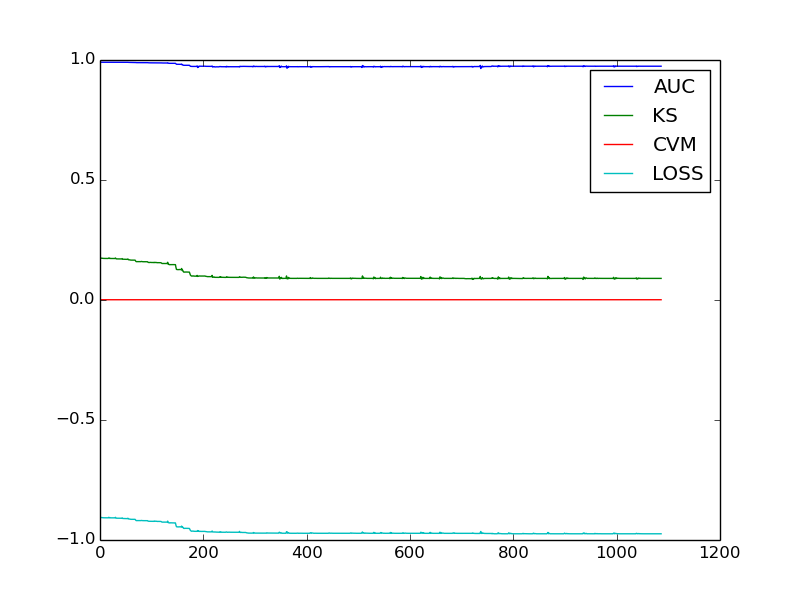
\includegraphics[width=.5\textwidth]{../imgs/transductor_stats_pt1.png}
	\caption{Performance of the ensemble of neural networks with homogeneous Dropout rate of $22$}
	\label{fig:dropout_22}
\end{figure}

\begin{figure}[!ht]
	\centering
	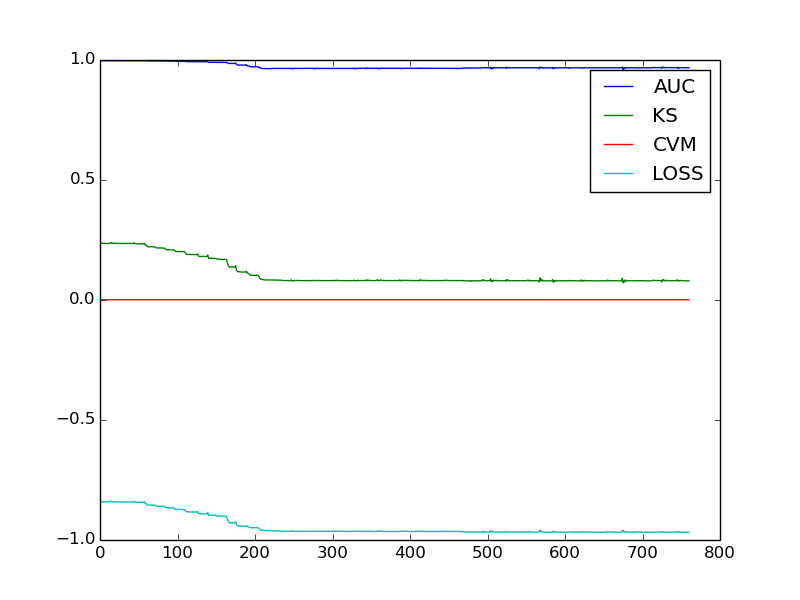
\includegraphics[width=.5\textwidth]{../imgs/transductor_stats_pt30.png}
	\caption{Performance of the ensemble of neural networks with heterogeneous Dropout rate of $22, 14.5 and 7$ }
	\label{fig:dropout_22_7}
\end{figure}

Secondly, we tested the length of pre-training for the transductor phase. To do so, the number of epochs ranged from 1 to 30.

\begin{figure}[!ht]
	\centering
	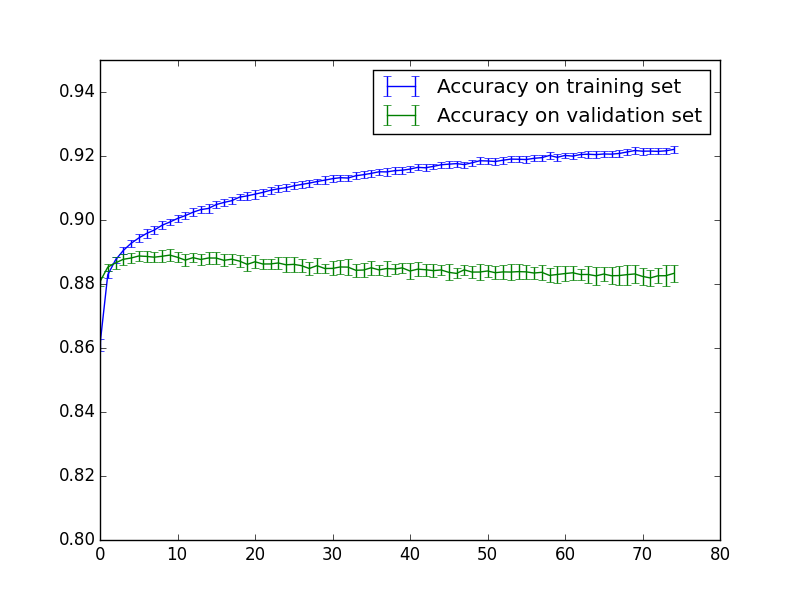
\includegraphics[width=.5\textwidth]{../imgs/ensemble_stats_d11.png}
	\caption{Performance of the ensemble of neural networks with the parameters
	and training algorithm described in Section~\ref{sec:system_design}.}
	\label{fig:ensemble_d11}
\end{figure}

\begin{figure}[!ht]
	\centering
	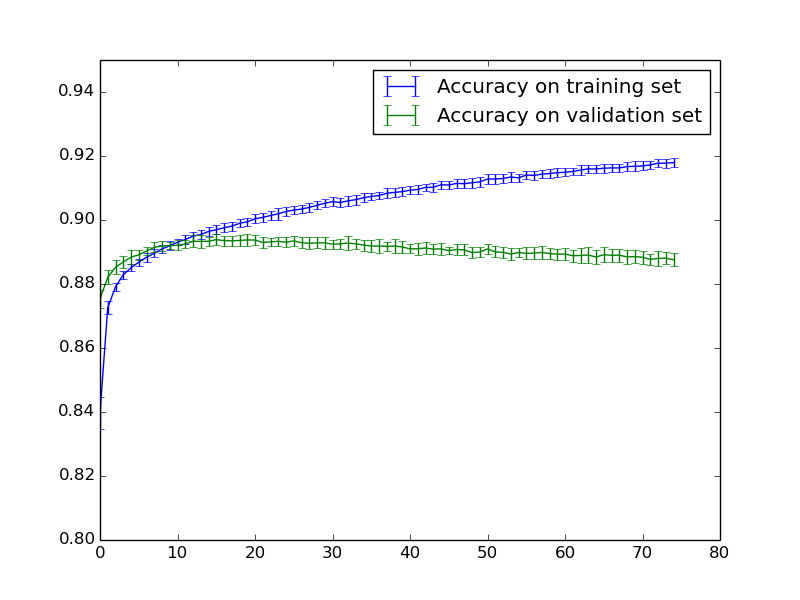
\includegraphics[width=.5\textwidth]{../imgs/ensemble_stats_d11_adadelta.png}
	\caption{Performance of the ensemble of neural networks with the parameters
	described in Section~\ref{sec:system_design}, a cross-entropy loss function
	and ADADELTA as optimization algorithm.}
	\label{fig:ensemble_d11_adadelta}
\end{figure}

We tried also changing the optimization algorithm used to train the model. Figure~\ref{fig:ensemble_d11} shows the performance of the ensemble of models
using the RMSProp algorithm, as described in Section \ref{sec:system_design}. In
Figure~\ref{fig:ensemble_d11_adadelta} instead we present the results for the
ADADELTA optimizer \cite{zeiler2012adadelta}. It is easy to see that the RMSProp
implementation outperforms ADADELTA on the training set, reaching higher
accuracy. The variance of the accuracy on the validation set is higher for
RMSProp which is probably a good thing for this kind of task, but more
noticeably, it does not degrade as fast as for the ADADELTA optimizer.

\begin{figure}[!ht]
	\centering
	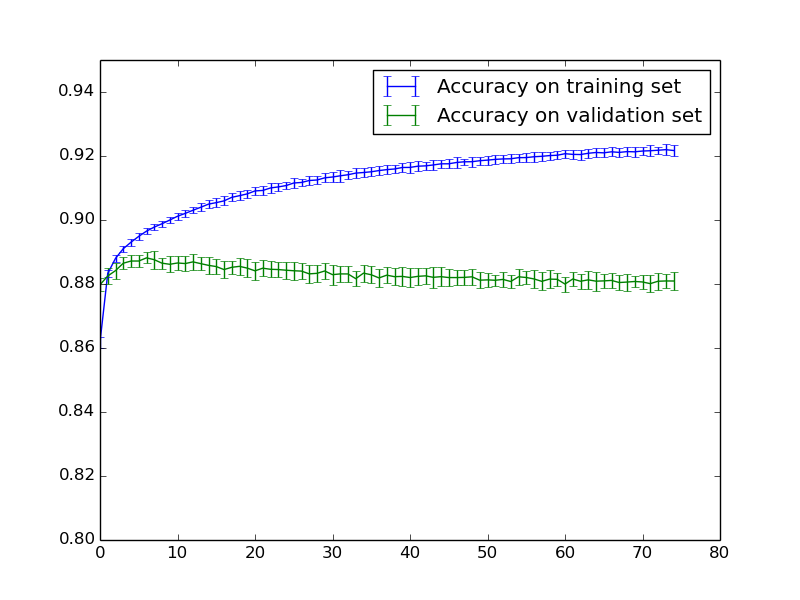
\includegraphics[width=.5\textwidth]{../imgs/ensemble_stats_d11_kld.png}
	\caption{Performance of the ensemble of neural networks with the parameters
	described in Section~\ref{sec:system_design} but the Kullback-Leibler
	Divergence as loss function.}
	\label{fig:ensemble_d11_kld}
\end{figure}

As for the loss function, we decided to experiment with the Kullback-Leibler
Divergence directly, as an alternative to the cross-entropy. The performance
results of the ensemble are given in Figure~\ref{fig:ensemble_d11_kld}. This
loss function performs slightly worse on the training set, and has a
significantly higher variance both on both data sets. However the negative slope
of the accuracy on the validation data is higher for this metric than that for
the cross-entropy.


\section{Conclusion}
\label{sec:conclusion}

\clearpage
\appendix

\section{Features for training}
\label{sec:features}
Follows a list of available features for training:
\begin{itemize}
	\item \texttt{FlightDistance}~-- distance between $\tau$ and PV (primary vertex, the
	original protons collision point);
	\item \texttt{FlightDistanceError}~-- error on FlightDistance;
	\item \texttt{mass}~-- reconstructed $\tau$ candidate invariant mass, which
	is \textit{absent in the test samples};
	\item \texttt{LifeTime}~-- life time of tau candidate;
	\item \texttt{IP}~-- Impact Parameter of tau candidate;
	\item \texttt{IPSig}~-- Significance of Impact Parameter;
	\item \texttt{VertexChi2}~-- $\chi^2$ of $\tau$ vertex;
	\item \texttt{dira}~-- cosine of the angle between the $\tau$ momentum and line
	between PV and tau vertex;
	\item \texttt{pt}~-- transverse momentum of $\tau$;
	\item \texttt{DOCAone}~-- Distance of Closest Approach between p0 and p1;
	\item \texttt{DOCAtwo}~-- Distance of Closest Approach between p1 and p2;
	\item \texttt{DOCAthree}~-- Distance of Closest Approach between p0 and p2;
	\item \texttt{IP\_p0p2}~-- Impact parameter of the p0 and p2 pair;
	\item \texttt{IP\_p1p2}~-- Impact parameter of the p1 and p2 pair;
	\item \texttt{isolationa}~-- track isolation variable;
	\item \texttt{isolationb}~-- track isolation variable;
	\item \texttt{isolationc}~-- track isolation variable;
	\item \texttt{isolationd}~-- track isolation variable;
	\item \texttt{isolatione}~-- track isolation variable;
	\item \texttt{isolationf}~-- track isolation variable;
	\item \texttt{iso}~-- track isolation variable;
	\item \texttt{CDF1}~-- cone isolation variable;
	\item \texttt{CDF2}~-- cone isolation variable;
	\item \texttt{CDF3}~-- cone isolation variable;
	\item \texttt{production}~-- source of $\tau$ (\textit{absent from test data});
	\item \texttt{ISO\_SumBDT}~-- track isolation variable;
	\item \texttt{p0\_IsoBDT}~-- track isolation variable;
	\item \texttt{p1\_IsoBDT}~-- track isolation variable;
	\item \texttt{p2\_IsoBDT}~-- track isolation variable;
	\item \texttt{p0\_track\_Chi2Dof}~-- quality of p0 muon track;
	\item \texttt{p1\_track\_Chi2Dof}~-- quality of p1 muon track;
	\item \texttt{p2\_track\_Chi2Dof}~-- quality of p2 muon track;
	\item \texttt{p0\_pt}~-- transverse momentum of p0 muon;
	\item \texttt{p0\_p}~-- momentum of p0 muon;
	\item \texttt{p0\_eta}~-- pseudorapidity of p0 muon;
	\item \texttt{p0\_IP}~-- Impact parameter of p0 muon;
	\item \texttt{p0\_IPSig}~-- Impact Parameter Significance of p0 muon;
	\item \texttt{p1\_pt}~-- transverse momentum of p1 muon;
	\item \texttt{p1\_p}~-- momentum of p1 muon;
	\item \texttt{p1\_eta}~-- pseudorapidity of p1 muon;
	\item \texttt{p1\_IP}~-- Impact parameter of p1 muon;
	\item \texttt{p1\_IPSig}~-- Impact Parameter Significance of p1 muon;
	\item \texttt{p2\_pt}~-- transverse momentum of p2 muon;
	\item \texttt{p2\_p}~-- momentum of p2 muon;
	\item \texttt{p2\_eta}~-- pseudorapidity of p2 muon;
	\item \texttt{p2\_IP}~-- Impact parameter of p2 muon;
	\item \texttt{p2\_IPSig}~-- Impact Parameter Significance of p2 muon;
	\item \texttt{SPDhits}~-- number of hits in the SPD detector;
	\item \texttt{min\_ANNmuon}~-- muon identification. LHCb collaboration trains
  	Artificial Neural Networks (ANN) from informations from RICH, ECAL,
  	HCAL, Muon system to distinguish muons from other particles. This
  	variable denotes the minimum of the three muons ANN. This feature
  	should not be used for training and is \textit{absent from the test
		sets};
	\item \texttt{signal}~-- is the target variable to predict.
\end{itemize}

%\printbibliography

\end{document}
